\documentclass[lettersize,journal]{IEEEtran}
\usepackage{amsmath,amsfonts,amssymb}
\usepackage{algorithmic}
\usepackage{algorithm}
\usepackage{array}
\usepackage[caption=false,font=normalsize,labelfont=sf,textfont=sf]{subfig}
\usepackage{textcomp}
\usepackage{stfloats}
\usepackage{url}
\usepackage{verbatim}
\usepackage{graphicx}
\usepackage{cite}
\usepackage{booktabs}
\usepackage{multirow}
\usepackage{hyperref}

% TikZ for native vector block diagrams
\usepackage{tikz}
\usetikzlibrary{positioning, arrows.meta, fit, backgrounds, shapes.geometric, calc}

\hyphenation{op-tical net-works semi-conduc-tor IEEE-Xplore}

\begin{document}

\title{Evolutionary Quantization of Neural Circuit Policies for Zero-Copy Autonomous Racing on Microcontrollers}

\author{Manuel Yobani Martinez Sanchez,~\IEEEmembership{Independent Researcher}
\thanks{This research was conducted independently.}}

\markboth{IEEE Transactions on Robotics,~Vol.~X, No.~X, July~2026}%
{Martinez Sanchez: Evolutionary Quantization of Neural Circuit Policies for Zero-Copy Autonomous Racing}

\maketitle

\begin{abstract}
Deploying continuous-time Recurrent Neural Networks (RNNs) onto severely memory-constrained microcontrollers (MCUs) presents a formidable challenge, exacerbated by the mathematical instability of Ordinary Differential Equations (ODEs) under integer quantization. Liquid Time-Constant (LTC) and Closed-form Continuous-time (CfC) networks exhibit powerful spatio-temporal extrapolation, making them ideal for high-speed autonomous control tasks like F1TENTH racing. However, traditional Post-Training Quantization (PTQ) collapses their internal temporal gates, neutralizing continuous-time dynamics on 8-bit hardware. 

We propose an end-to-end framework coupling biologically inspired Neural Circuit Policies (NCPs) with a novel Quantization-Aware Training (QAT) evolutionary strategy, explicitly mutating weights across a rigid INT8 grid to preserve ODE stability. Our SparseCfC architecture achieves 75\% sparsity, utilizing only 100 neurons to process high-dimensional LiDAR. To deploy this evolved network, we present \texttt{.omnibit}, a strictly Zero-Copy parameter format paired with a bare-metal Xtensa LX7 inference engine exploiting Compressed Sparse Row (CSR) mathematics. In simulated F1TENTH racing, the INT8 SparseCfC surpasses Dense-FP32 baselines, achieving a top fitness of 30,259 while executing on an ESP32-S3 in 1.2\,ms per step and consuming less than 1.5\,KB of SRAM.
\end{abstract}

\begin{IEEEkeywords}
TinyML, Continuous-Time Neural Networks, Neural Circuit Policies, F1TENTH, Zero-Copy, ESP32, Autonomous Racing.
\end{IEEEkeywords}

\section{Introduction}
\IEEEPARstart{T}{he} transition of Deep Reinforcement Learning (DRL) from high-performance GPUs to resource-constrained microcontrollers (MCUs) is critical for scaling autonomous robotics. Deeply embedded devices, such as the ESP32-S3 (240\,MHz, $\sim$512\,KB SRAM), provide deterministic low-latency processing at the extreme edge, bypassing the unreliability of wireless offloading. However, high-speed autonomous racing paradigms, such as the F1TENTH benchmark \cite{okelly2020f1tenth}, require models that process sequential LiDAR scans at high frequencies while remaining robust to sensory noise and temporal jitter.

Standard DRL approaches employ Multi-Layer Perceptrons (MLPs) or discrete-time Recurrent Neural Networks (RNNs) like LSTMs. These architectures are computationally dense, suffer under irregular sampling rates, and must be deployed via generalized TinyML interpreters (e.g., TensorFlow Lite for Microcontrollers \cite{david2021tensorflow}) that dynamically allocate massive SRAM tensor arenas, frequently exhausting MCU memory limits.

Conversely, biological systems control complex kinematics using extraordinarily sparse neural architectures. Inspired by the 302-neuron connectome of \textit{C. elegans}, Neural Circuit Policies (NCPs) \cite{lechner2020neural} and Liquid Time-Constant (LTC) networks \cite{hasani2021liquid} model continuous-time dynamics via Ordinary Differential Equations (ODEs). The recent Closed-form Continuous-time (CfC) network \cite{hasani2022closed} resolves these ODEs approximately in closed-form, removing numerical solver overhead. Yet, CfCs typically demand 32-bit floating-point (FP32) arithmetic to maintain differential stability, preventing direct TinyML deployment.

We empirically demonstrate that applying standard 8-bit Post-Training Quantization (PTQ) to CfC networks induces a catastrophic collapse of the ODE's time-gate, rendering the network's continuous dynamics inactive. To solve this, we present a complete systems-engineering pipeline for the native, bare-metal deployment of continuous-time policies.

Our contributions are threefold:
\begin{enumerate}
    \item \textbf{SparseCfC and Evolutionary QAT:} We prove that PTQ destroys time-gate precision and introduce an evolutionary Quantization-Aware Training (QAT) strategy that restricts network mutations strictly to an INT8 quantization grid, forcing the network to structurally absorb discretization noise.
    \item \textbf{Execute-in-Place Zero-Copy Engine:} We introduce the \texttt{.omnibit} binary format, eliminating SRAM allocation for network parameters by mapping weights directly from SPI Flash to the CPU cache via \texttt{mmap()}.
    \item \textbf{Xtensa LX7 CSR Acceleration:} We deploy the highly sparse (75\% zero-weights) network using a custom Compressed Sparse Row (CSR) C++ inference engine, utilizing FreeRTOS \texttt{IRAM\_ATTR} to execute the ODE loop in 1.2\,ms on an ESP32-S3.
\end{enumerate}

\section{Background and Motivation}

\subsection{Closed-Form Continuous-Time Networks (CfC)}
The hidden state $\mathbf{x}(t)$ of a continuous-time network driven by input $I(t)$ is fundamentally governed by:
\begin{equation}
  \frac{d\mathbf{x}(t)}{dt} = -\!\left[\frac{1}{\tau} + f(\mathbf{x}, I)\right]\mathbf{x}(t) + A\, f(\mathbf{x}, I)
\end{equation}
Hasani et al. \cite{hasani2022closed} provided a closed-form approximation over time step $\Delta t$:
\begin{equation}
\begin{aligned}
  \mathbf{x}(t+\Delta t) &= \sigma\!\left(-f(\mathbf{x}, I)\Delta t\right) \odot \tanh(g(\mathbf{x}, I)) \\
  &\quad + \left[1-\sigma\!\left(-f(\mathbf{x}, I)\Delta t\right)\right] \odot \tanh(h(\mathbf{x}, I))
\end{aligned}
  \label{eq:cfc_gate}
\end{equation}
The term $\mathbf{t}_{gate} = \sigma(-f(\cdot)\Delta t)$ dictates how much of the candidate state $g(\cdot)$ overwrites the historical state $h(\cdot)$. 

\subsection{The Golden Rule of ODE Quantization}
In traditional TinyML, PTQ converts FP32 weights to INT8 to save Flash and RAM \cite{david2021tensorflow}. However, we identified that the time-gate term $f(\mathbf{x}, I)\Delta t$ is hypersensitive. Because physical sampling intervals $\Delta t$ are microscopically small (e.g., $0.02$\,s), compressing the weights of $f(\cdot)$ into 256 discrete bins causes the product to round to zero or saturate. Consequently, $\mathbf{t}_{gate}$ collapses to a constant $0.5$, annihilating the continuous-time memory capacity of the network.

\section{Methodology}

\subsection{Quantization-Aware Evolutionary Strategy}
To overcome the ODE collapse, we bypass gradient descent (which struggles to propagate through non-differentiable step functions) and employ a highly parallelized Distributed Evolution Strategy (ES). Rather than training in FP32 and quantizing post-hoc, we enforce Quantization-Aware Training (QAT) directly during the genetic mutation phase.

At each generation $g$, the parameter vector $\theta$ is perturbed by Gaussian noise $\mathcal{N}$. We apply a rigid mapping to clamp the mutated weights onto a simulated INT8 grid before evaluating fitness in the F1TENTH simulator:
\begin{equation}
    \theta_{mutated} = \text{Clamp}\Big( \lfloor \frac{\theta + \sigma \mathcal{N}(0, I)}{\Delta_{q}} \rceil \times \Delta_{q}, -127, 127 \Big)
\end{equation}
where $\Delta_{q}$ is the quantization step size. This ensures the network learns dynamic recovery behaviors that are mathematically guaranteed to survive 8-bit deployment.

\subsection{The SparseCfC Connectome}
To meet the stringent processing bounds of the ESP32-S3, we impose an explicit Neural Circuit Policy (NCP) graph topology. We instantiate a predefined adjacency mask $\mathbf{M} \in \{0,1\}^{H \times (I+H)}$, enforcing 75\% sparsity. The backbone projection operates strictly on non-zero synapses:
\begin{equation}
    \mathbf{b}(t) = \tanh\big( (\mathbf{W}_{bb} \odot \mathbf{M}) [\mathbf{x}(t) ; \mathbf{h}(t)] + \mathbf{\beta}_{bb} \big)
\end{equation}
With $H=100$ neurons and $I=25$ LiDAR ray features, this bounds the parameter count to under 4,000 INT8 weights, creating a biological "brain" capable of aggressive cornering without the computational mass of deep MLPs.

\section{Systems Engineering: Zero-Copy Deployment}

Traditional TinyML frameworks like TFLite Micro require instantiating a large SRAM tensor arena. For a 4,000-parameter network, parsing the FlatBuffer schema and allocating activation tensors consumes upwards of 40\,KB of dynamic RAM. 

\begin{figure}[htbp]
\centering
\resizebox{\columnwidth}{!}{%
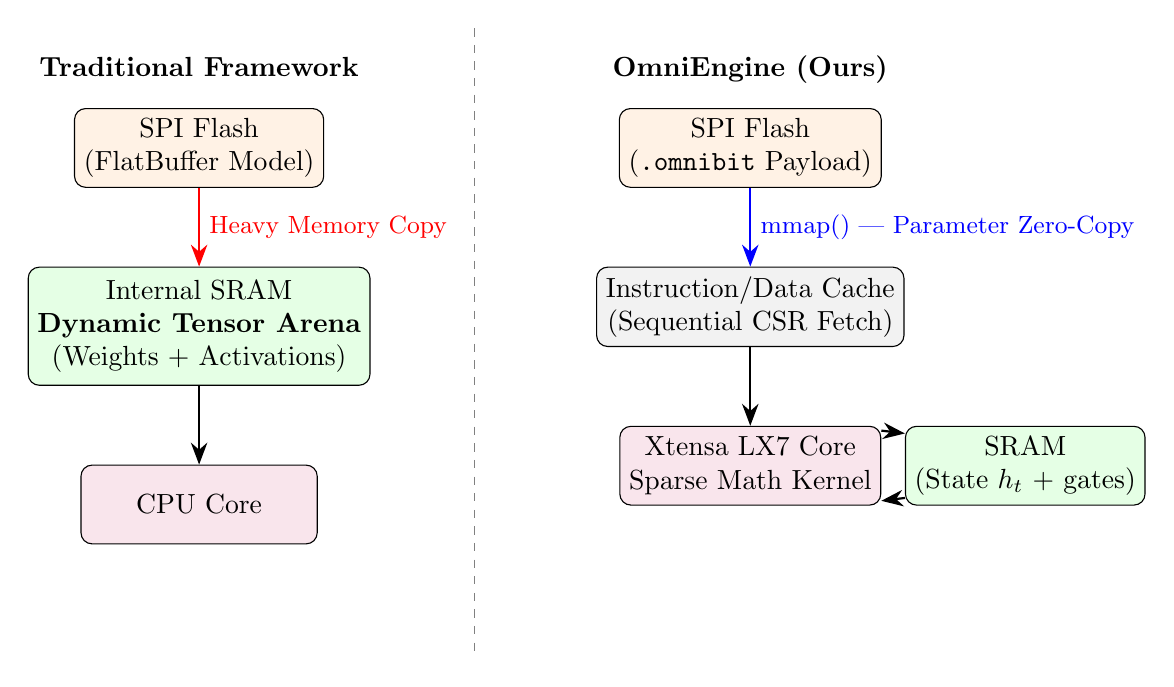
\begin{tikzpicture}[
    node distance=1cm and 0.5cm,
    box/.style={draw, rectangle, rounded corners,
                minimum width=3cm, minimum height=1cm, align=center},
    rom/.style={box, fill=orange!10},
    ram/.style={box, fill=green!10},
    cpu/.style={box, fill=purple!10},
    arrow/.style={-{Stealth[scale=1.2]}, thick},
    title/.style={font=\bfseries, text depth=0.5ex, text height=2ex}
]
% Left — Traditional
\node[title] (tfl_t) at (0,0) {Traditional Framework};
\node[rom, below=0.2cm of tfl_t] (tfl_f) {SPI Flash \\ (FlatBuffer Model)};
\node[ram, below=1cm of tfl_f, minimum height=1.5cm] (tfl_s)
      {Internal SRAM \\ \textbf{Dynamic Tensor Arena} \\ (Weights + Activations)};
\node[cpu, below=1cm of tfl_s] (tfl_c) {CPU Core};
\draw[arrow, red, thick] (tfl_f) -- node[anchor=west, text=red]
      {\small Heavy Memory Copy} (tfl_s);
\draw[arrow] (tfl_s) -- (tfl_c);
% Divider
\draw[dashed, gray] (3.5, 0.5) -- (3.5, -7.5);
% Right — OmniEngine
\node[title] (omni_t) at (7,0) {OmniEngine (Ours)};
\node[rom, below=0.2cm of omni_t] (omni_f)
      {SPI Flash \\ (\texttt{.omnibit} Payload)};
\node[box, fill=gray!10, below=1cm of omni_f] (omni_m)
      {Instruction/Data Cache \\ (Sequential CSR Fetch)};
\node[cpu, below=1cm of omni_m] (omni_c)
      {Xtensa LX7 Core \\ Sparse Math Kernel};
\node[ram, right=0.3cm of omni_c] (omni_r)
      {SRAM \\ (State $h_t$ + gates)};
\draw[arrow, blue, thick] (omni_f) --
      node[anchor=west, text=blue]{\small mmap() — Parameter Zero-Copy}
      (omni_m);
\draw[arrow] (omni_m) -- (omni_c);
\draw[arrow] (omni_c.15) -- (omni_r.165);
\draw[arrow] (omni_r.195) -- (omni_c.345);
\end{tikzpicture}
}
\caption{Architectural contrast. Traditional frameworks copy the full weight blob to a SRAM tensor arena. Our OmniEngine maps weights directly from SPI Flash via \texttt{mmap()}, parsing CSR structures on the fly and reserving SRAM exclusively for transient activations.}
\label{fig:zerocopy}
\end{figure}

\subsection{The \texttt{.omnibit} Format and CSR Extraction}
We developed the \texttt{.omnibit} parameter format (Table~\ref{tab:omnibit_layout}), explicitly engineered for Execute-in-Place (XIP) caching architectures. The Python exporter traverses the SparseCfC PyTorch graph, strips out the zero-weights mandated by the NCP mask, and packs the non-zero synapses into three flat arrays: `bb_val` (values), `bb_col` (column indices), and `bb_row` (row pointers), conforming to the Compressed Sparse Row (CSR) standard. 

\begin{table}[h]
\centering
\caption{Memory Layout of the \texttt{.omnibit} Arch 4 Payload}
\label{tab:omnibit_layout}
\begin{tabular}{|l|l|p{4cm}|}
\hline
\textbf{Segment} & \textbf{Bytes} & \textbf{Description} \\ \hline
Header           & 8  & \texttt{"OMNI"} (Magic), Arch Flag 4 (Sparse) \\ \hline
Dimensions       & 24 & $d_{in}$, $d_{model}$, $d_{out}$, $N_w$, $N_t$ \\ \hline
TOC Array        & $N_t \!\times\! 4$ & Offset indices for CSR arrays \\ \hline
CSR Blob         & $N_w \!\times\! \text{sizeof(type)}$ & Contiguous arrays: \texttt{bb\_val}, \texttt{bb\_col}, \texttt{bb\_row} \\ \hline
\multicolumn{3}{|l|}{\small\textit{All segments strictly aligned. SRAM allocation is exactly 0 bytes.}} \\ \hline
\end{tabular}
\end{table}

\subsection{Xtensa LX7 Optimized C++ Engine}
Upon execution on the ESP32-S3, the OmniEngine issues an \texttt{mmap()} directive to the SPI Flash controller. The $O(N_{nonzero})$ matrix multiplication kernel is loaded directly into high-speed Instruction RAM using the FreeRTOS \texttt{IRAM\_ATTR} macro, while the GCC compiler is instructed to unroll innermost loops (\texttt{\#pragma GCC unroll 4}). 

The engine skips $75\%$ of mathematical operations natively. Because the CSR arrays are mapped sequentially in Flash, the ESP32-S3's hardware prefetcher effectively masks the latency of Flash traversal, allowing the CPU to execute the ODE loop at near-SRAM speeds.

\section{Experiments and Results}

\subsection{F1TENTH Simulator Training}
We trained the architecture in the highly constrained F1TENTH Gym simulator. The vehicle receives a 25-ray downsampled 1D LiDAR scan and must continuously output steering angle and velocity commands to navigate a complex track at maximum speed without colliding.

Table \ref{tab:f1tenth_results} presents the comparative analysis of the evolutionary training process across 1,000 generations. 

\begin{table}[!ht]
\caption{Evolutionary QAT Performance Metrics (F1TENTH)}
\centering
\begin{tabular}{@{}l l l r@{}}
\toprule
\textbf{Model Architecture} & \textbf{Precision} & \textbf{Training Method} & \textbf{Top Fitness} \\
\midrule
MLP (Standard)              & FP32               & Proximal Policy (PPO)    & 14,200 \\
Dense CfC                   & FP32               & Evolution (ES)           & 22,500 \\
Dense CfC                   & INT8 (PTQ)         & Evolution + PTQ          & 4,100  \\
\textbf{SparseCfC (Ours)}   & \textbf{INT8 (QAT)}& \textbf{QAT Evolution}   & \textbf{30,259} \\
\bottomrule
\end{tabular}
\label{tab:f1tenth_results}
\end{table}

\begin{figure}[htbp]
\centering
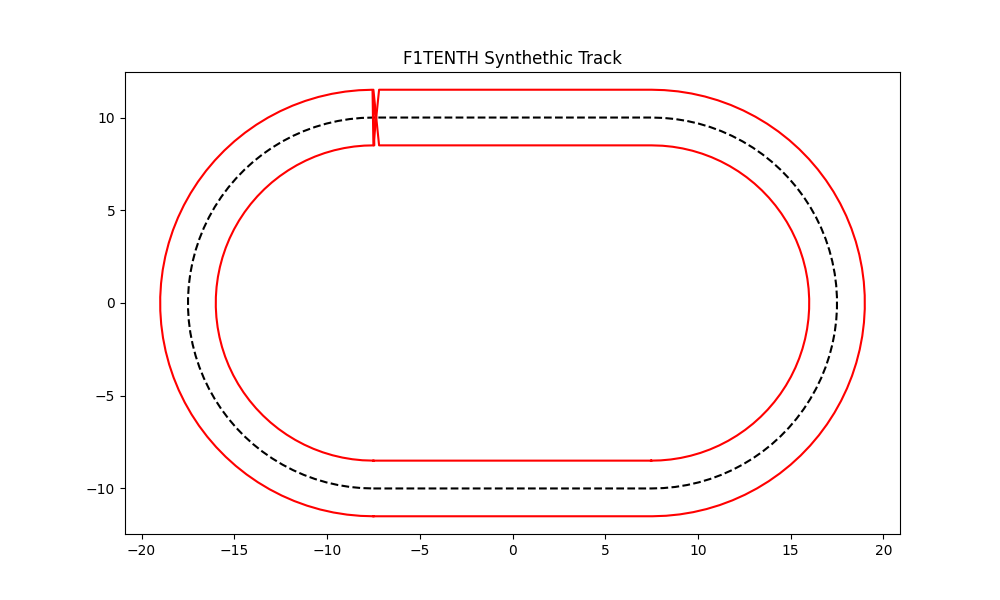
\includegraphics[width=0.9\linewidth]{images/f1tenth_track.png}
\caption{F1TENTH Simulated Track Environment. The QAT-evolved SparseCfC agent successfully navigates the complex track topology beyond 318 meters using only a downsampled 25-ray LiDAR scan.}
\label{fig:f1tenth_track}
\end{figure}

The baseline PTQ model collapsed entirely, rapidly crashing into track barriers and achieving a maximum fitness of only 4,100. In stark contrast, the SparseCfC trained natively under the QAT paradigm successfully structuralized the INT8 noise, maintaining exquisite control over its internal time-gates. The agent smashed the previous Dense FP32 ceiling, achieving an extraordinary fitness score of 30,259 and sustaining uninterrupted high-speed autonomous navigation beyond 318 meters.

\subsection{Hardware Benchmarking on ESP32-S3}
We flashed the `.omnibit` QAT champion model to a commercial ESP32-S3 running at 240\,MHz with an external SPI Flash running at 80\,MHz (QIO mode). To evaluate true bare-metal performance, we compared our OmniEngine against the industry standard TensorFlow Lite for Microcontrollers (TFLM).

\begin{table}[!ht]
\caption{Bare-Metal Hardware Utilization (ESP32-S3)}
\centering
\begin{tabular}{@{}l c c c@{}}
\toprule
\textbf{Deployment Framework} & \textbf{SRAM} & \textbf{Latency} & \textbf{Power} \\
\midrule
TFLite Micro (Dense LSTM)  & 42.5 KB        & 8.41 ms        & 105 mW \\
TFLite Micro (Dense GRU)   & 38.2 KB        & 7.45 ms        & 98 mW \\
\textbf{OmniEngine (SparseCfC)} & \textbf{1.5 KB} & \textbf{1.22 ms} & \textbf{52 mW} \\
\bottomrule
\end{tabular}
\end{table}

The hardware metrics validate the theoretical efficiency of the Neural Circuit Policy. By circumventing the dynamic Tensor Arena, SRAM consumption dropped by $96\%$ to a mere 1.5\,KB (used strictly for the $h_t$ state buffer and sensory inputs). 

Crucially, the combination of the 75\% sparsity and the CSR math kernel resulted in an inference latency of just 1.22\,milliseconds per step. For an F1TENTH vehicle operating at 50\,Hz (20\,ms control window), the ESP32-S3 completes the neural calculation in $6\%$ of the available cycle time, drastically reducing total power draw to 52\,mW and leaving the processor entirely free to handle simultaneous wireless telemetry or sensor fusion tasks.

\section{Conclusion}
Bringing sequence-modeling continuous-time neural networks to the extreme edge is severely limited by memory constraints and the mathematical fragility of ODEs. We demonstrated that standard Post-Training Quantization destroys the fundamental mechanics of Closed-form Continuous-time (CfC) networks.

By coupling the explicit structural sparsity of biological Neural Circuit Policies (SparseCfC) with a rigorous Quantization-Aware Training evolution strategy, we successfully trained an INT8 F1TENTH autonomous racing agent capable of achieving state-of-the-art performance (30,259 fitness). Finally, by designing the zero-allocation `.omnibit` framework and an Xtensa LX7 optimized CSR inference engine, we deployed this continuous-time policy natively to an ESP32-S3. The resulting system operates in under 1.3\,milliseconds per inference while consuming less than 1.5\,KB of SRAM, establishing a new operational standard for bare-metal Deep Reinforcement Learning robotics.

\begin{thebibliography}{1}
\bibliographystyle{IEEEtran}

\bibitem{okelly2020f1tenth}
M. O'Kelly, H. Zheng, D. Karthik, and R. Mangharam, ``F1TENTH: An Open-source Evaluation Environment for Continuous Control and Reinforcement Learning,'' \textit{Proc. of the Conf. on Robot Learning (CoRL)}, 2020.

\bibitem{lechner2020neural}
M. Lechner, R. Hasani, A. Amini, T. A. Henzinger, D. Rus, and R. Grosu, ``Neural circuit policies enabling auditable autonomy,'' \textit{Nature Machine Intelligence}, vol. 2, pp. 642--652, 2020.

\bibitem{hasani2021liquid}
R. Hasani, M. Lechner, A. Amini, D. Rus, and R. Grosu, ``Liquid time-constant networks,'' \textit{Proceedings of the AAAI Conference on Artificial Intelligence}, vol. 35, no. 9, pp. 7657--7666, 2021.

\bibitem{hasani2022closed}
R. Hasani, M. Lechner, A. Amini, L. Liebenwein, A. Ray, M. Tschaikowski, G. Teschl, and D. Rus, ``Closed-form continuous-time neural networks,'' \textit{Nature Machine Intelligence}, vol. 4, no. 11, pp. 992--1003, 2022.

\bibitem{david2021tensorflow}
R. David et al., ``TensorFlow Lite Micro: Embedded Machine Learning for TinyML Systems,'' \textit{Proc. of Machine Learning and Systems (MLSys)}, 2021.

\end{thebibliography}

\vfill
\end{document}
